% Options for packages loaded elsewhere
\PassOptionsToPackage{unicode}{hyperref}
\PassOptionsToPackage{hyphens}{url}
%
\documentclass[
]{article}
\usepackage{amsmath,amssymb}
\usepackage{lmodern}
\usepackage{iftex}
\ifPDFTeX
  \usepackage[T1]{fontenc}
  \usepackage[utf8]{inputenc}
  \usepackage{textcomp} % provide euro and other symbols
\else % if luatex or xetex
  \usepackage{unicode-math}
  \defaultfontfeatures{Scale=MatchLowercase}
  \defaultfontfeatures[\rmfamily]{Ligatures=TeX,Scale=1}
\fi
% Use upquote if available, for straight quotes in verbatim environments
\IfFileExists{upquote.sty}{\usepackage{upquote}}{}
\IfFileExists{microtype.sty}{% use microtype if available
  \usepackage[]{microtype}
  \UseMicrotypeSet[protrusion]{basicmath} % disable protrusion for tt fonts
}{}
\makeatletter
\@ifundefined{KOMAClassName}{% if non-KOMA class
  \IfFileExists{parskip.sty}{%
    \usepackage{parskip}
  }{% else
    \setlength{\parindent}{0pt}
    \setlength{\parskip}{6pt plus 2pt minus 1pt}}
}{% if KOMA class
  \KOMAoptions{parskip=half}}
\makeatother
\usepackage{xcolor}
\usepackage[margin=1in]{geometry}
\usepackage{graphicx}
\makeatletter
\def\maxwidth{\ifdim\Gin@nat@width>\linewidth\linewidth\else\Gin@nat@width\fi}
\def\maxheight{\ifdim\Gin@nat@height>\textheight\textheight\else\Gin@nat@height\fi}
\makeatother
% Scale images if necessary, so that they will not overflow the page
% margins by default, and it is still possible to overwrite the defaults
% using explicit options in \includegraphics[width, height, ...]{}
\setkeys{Gin}{width=\maxwidth,height=\maxheight,keepaspectratio}
% Set default figure placement to htbp
\makeatletter
\def\fps@figure{htbp}
\makeatother
\setlength{\emergencystretch}{3em} % prevent overfull lines
\providecommand{\tightlist}{%
  \setlength{\itemsep}{0pt}\setlength{\parskip}{0pt}}
\setcounter{secnumdepth}{-\maxdimen} % remove section numbering
\ifLuaTeX
  \usepackage{selnolig}  % disable illegal ligatures
\fi
\IfFileExists{bookmark.sty}{\usepackage{bookmark}}{\usepackage{hyperref}}
\IfFileExists{xurl.sty}{\usepackage{xurl}}{} % add URL line breaks if available
\urlstyle{same} % disable monospaced font for URLs
\hypersetup{
  pdftitle={Paradigma de población en declive},
  pdfauthor={BIOL4558},
  hidelinks,
  pdfcreator={LaTeX via pandoc}}

\title{Paradigma de población en declive}
\author{BIOL4558}
\date{Agosto 2021}

\begin{document}
\maketitle

{
\setcounter{tocdepth}{2}
\tableofcontents
}
\textbf{P }: ¿Es la tasa intrínseca de crecimiento \(r_{max}\) positiva
o negativa para la mayoría de las especies de la tierra? ¿¿¿Por qué???

\textbf{P }: Dado que la mayoría de las especies son capaces de crecer
de forma sostenida y alcanzar un gran tamaño de población en condiciones
favorables, ¿cómo se reducen las poblaciones en primer lugar? ¿Por qué
están disminuyendo muchas poblaciones a pesar de su capacidad intrínseca
de crecer? ¿Es todo aleatorio o es más sistemático?

\hypertarget{amenazas-a-las-poblaciones}{%
\subsection{Amenazas a las
poblaciones}\label{amenazas-a-las-poblaciones}}

La respuesta, por supuesto, es que la capacidad intrínseca de crecer en
condiciones ideales no es toda la historia. Las poblaciones son
existencias con entradas y salidas, y si la mortalidad excede los
nacimientos \emph{en las condiciones actuales }, la población disminuirá
hasta que se inviertan estas condiciones desfavorables.

En la conferencia del ``paradigma de la pequeña población'', discutimos
varias \textbf{amenazas estocásticas } para las poblaciones, incluida la
pérdida de diversidad genética (deriva genética), la estocasticidad
demográfica y los eventos ambientales catastróficos. Estas amenazas solo
afectan realmente a poblaciones pequeñas. Las grandes poblaciones son en
su mayoría resistentes a las amenazas estocásticas.

¡Sin embargo, las grandes poblaciones también pueden verse amenazadas!
Los factores que amenazan a grandes poblaciones generalmente se
denominan \textbf{amenazas deterministas }.

El \textbf{paradigma de la población en declive } se centra en los
factores que hacen que las grandes poblaciones sean pequeñas, es decir,
es el \emph{estudio de los procesos deterministas que provocan el
declive de la población (que inclinan la balanza y provocan que las
muertes superen los nacimientos), y cómo estos procesos pueden
revertirse mediante una gestión de conservación eficaz}.

¿Cuáles son algunos de los factores que pueden \emph{inclinar la
balanza} por así decirlo, de modo que las poblaciones en crecimiento o
estables se conviertan en poblaciones en declive?

\hypertarget{cosecha-excesiva}{%
\subsubsection{Cosecha excesiva}\label{cosecha-excesiva}}

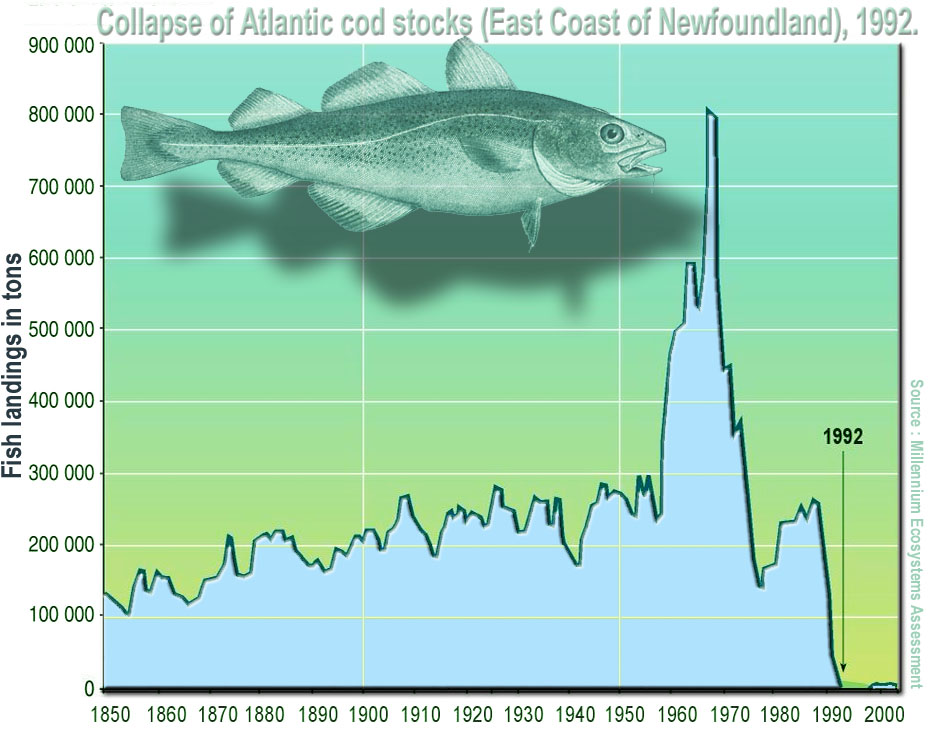
\includegraphics{figures/overharvest1.jpg}

\hypertarget{puxe9rdida-y-degradaciuxf3n-del-huxe1bitat}{%
\subsubsection{Pérdida y degradación del
hábitat}\label{puxe9rdida-y-degradaciuxf3n-del-huxe1bitat}}

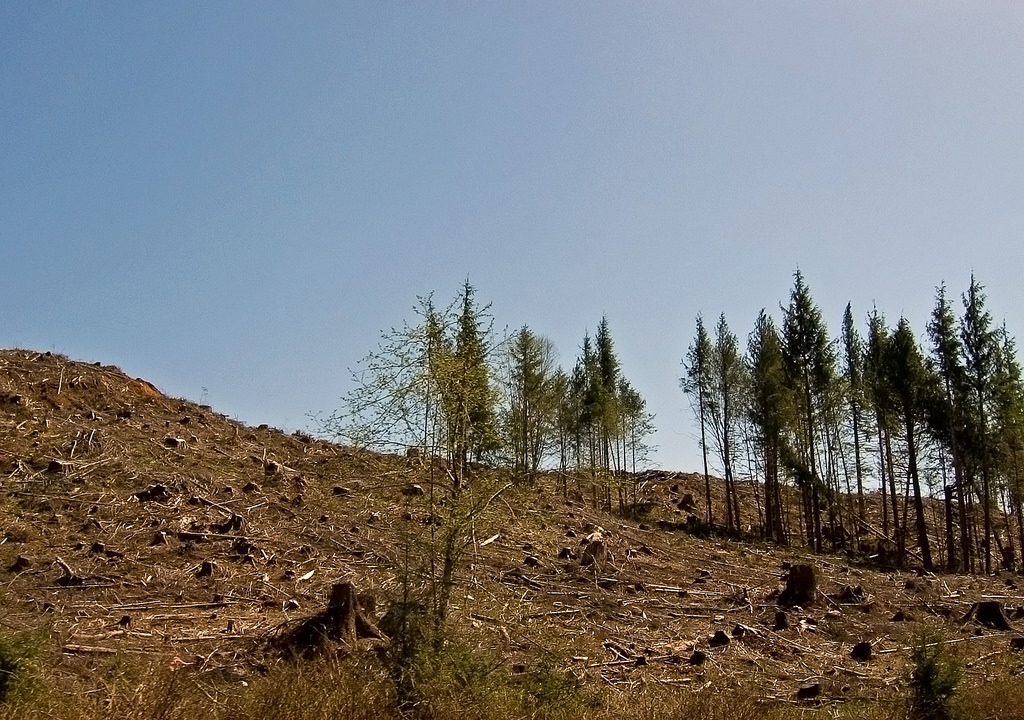
\includegraphics{figures/habitatloss1.jpg}

\hypertarget{patuxf3genos-y-paruxe1sitos}{%
\subsubsection{Patógenos y
parásitos}\label{patuxf3genos-y-paruxe1sitos}}

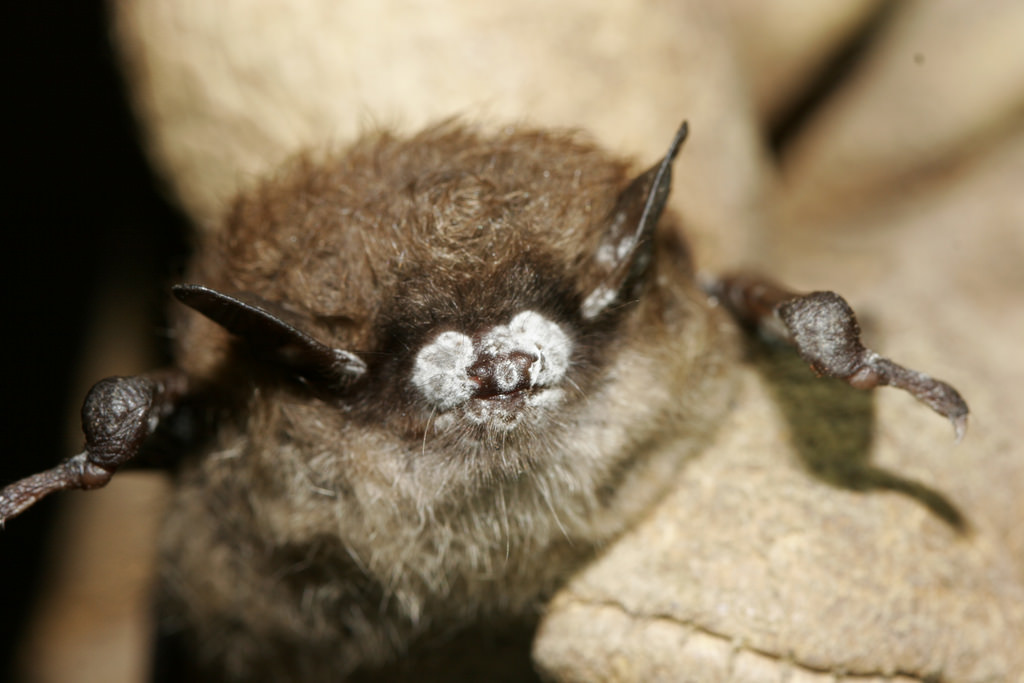
\includegraphics{figures/whitenose1.jpg}

\hypertarget{cambio-climuxe1tico}{%
\subsubsection{Cambio climático}\label{cambio-climuxe1tico}}

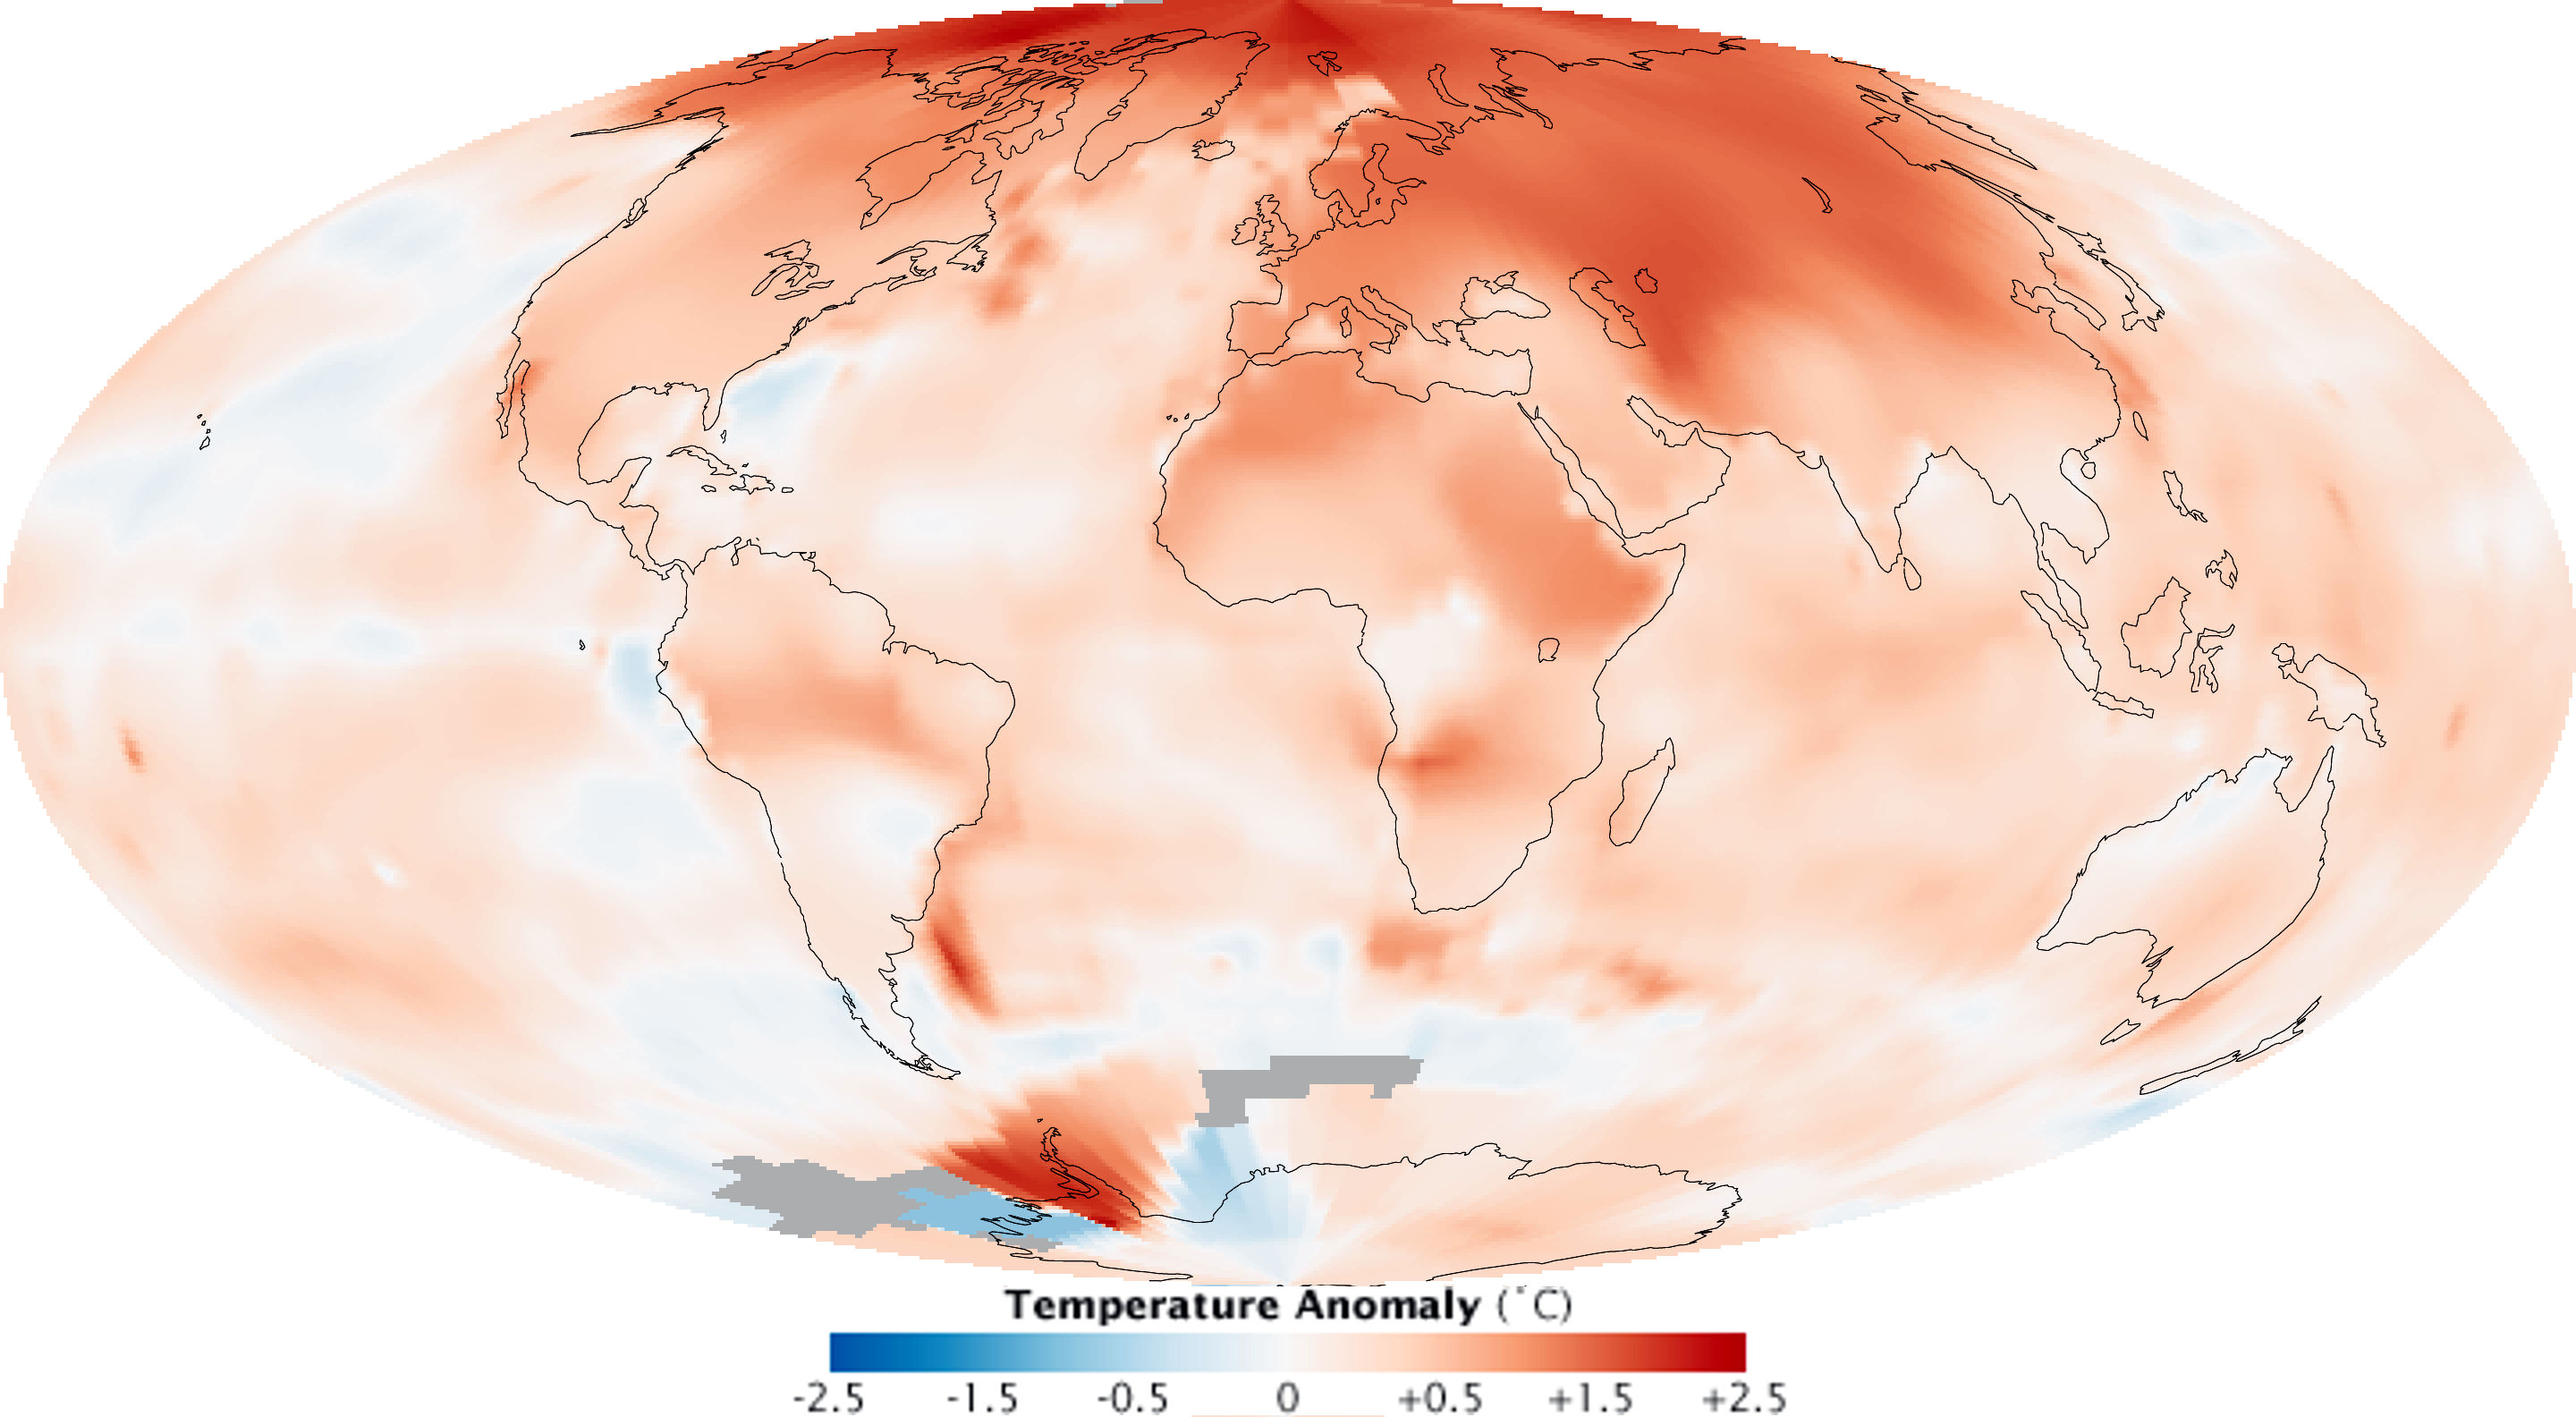
\includegraphics{figures/climatechange1.jpg}

Este mapa muestra la diferencia (anomalía) entre las temperaturas
actuales y las temperaturas medias (normales) registradas desde 1880.

\hypertarget{especies-exuxf3ticas-invasoras}{%
\subsubsection{Especies exóticas
invasoras}\label{especies-exuxf3ticas-invasoras}}

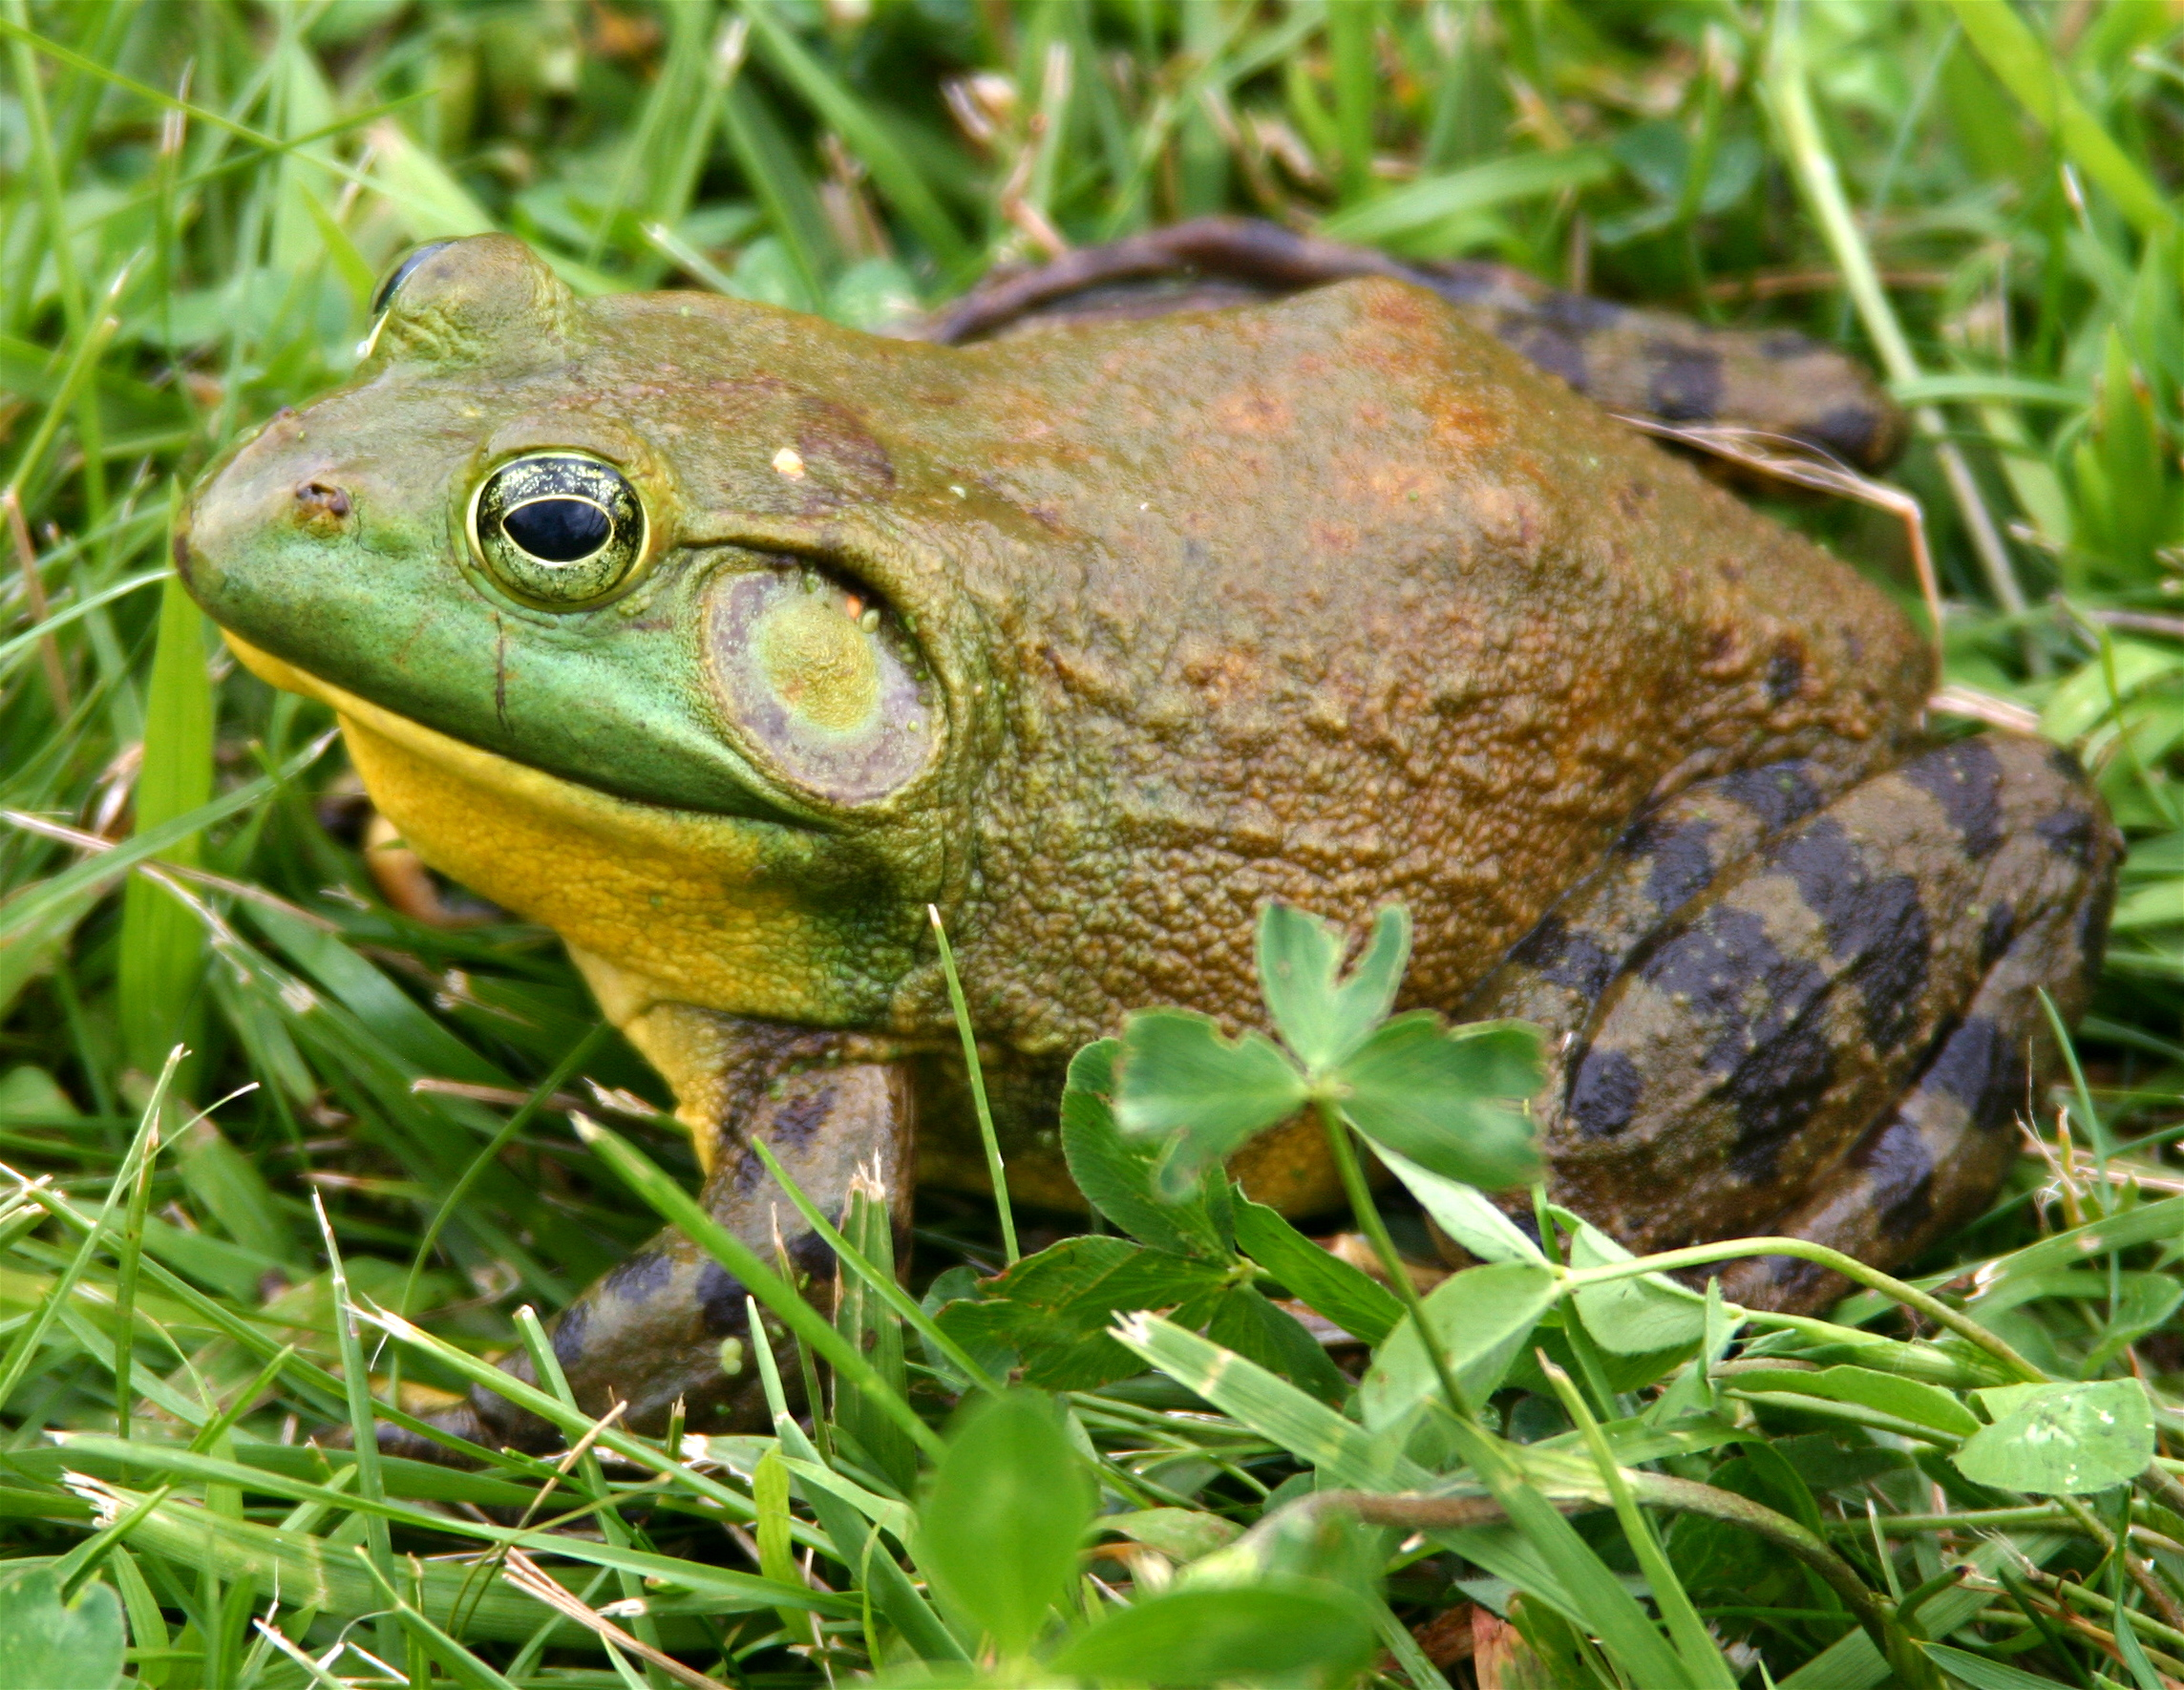
\includegraphics{figures/bullfrog1.jpg}

\hypertarget{contaminaciuxf3n}{%
\subsubsection{Contaminación}\label{contaminaciuxf3n}}

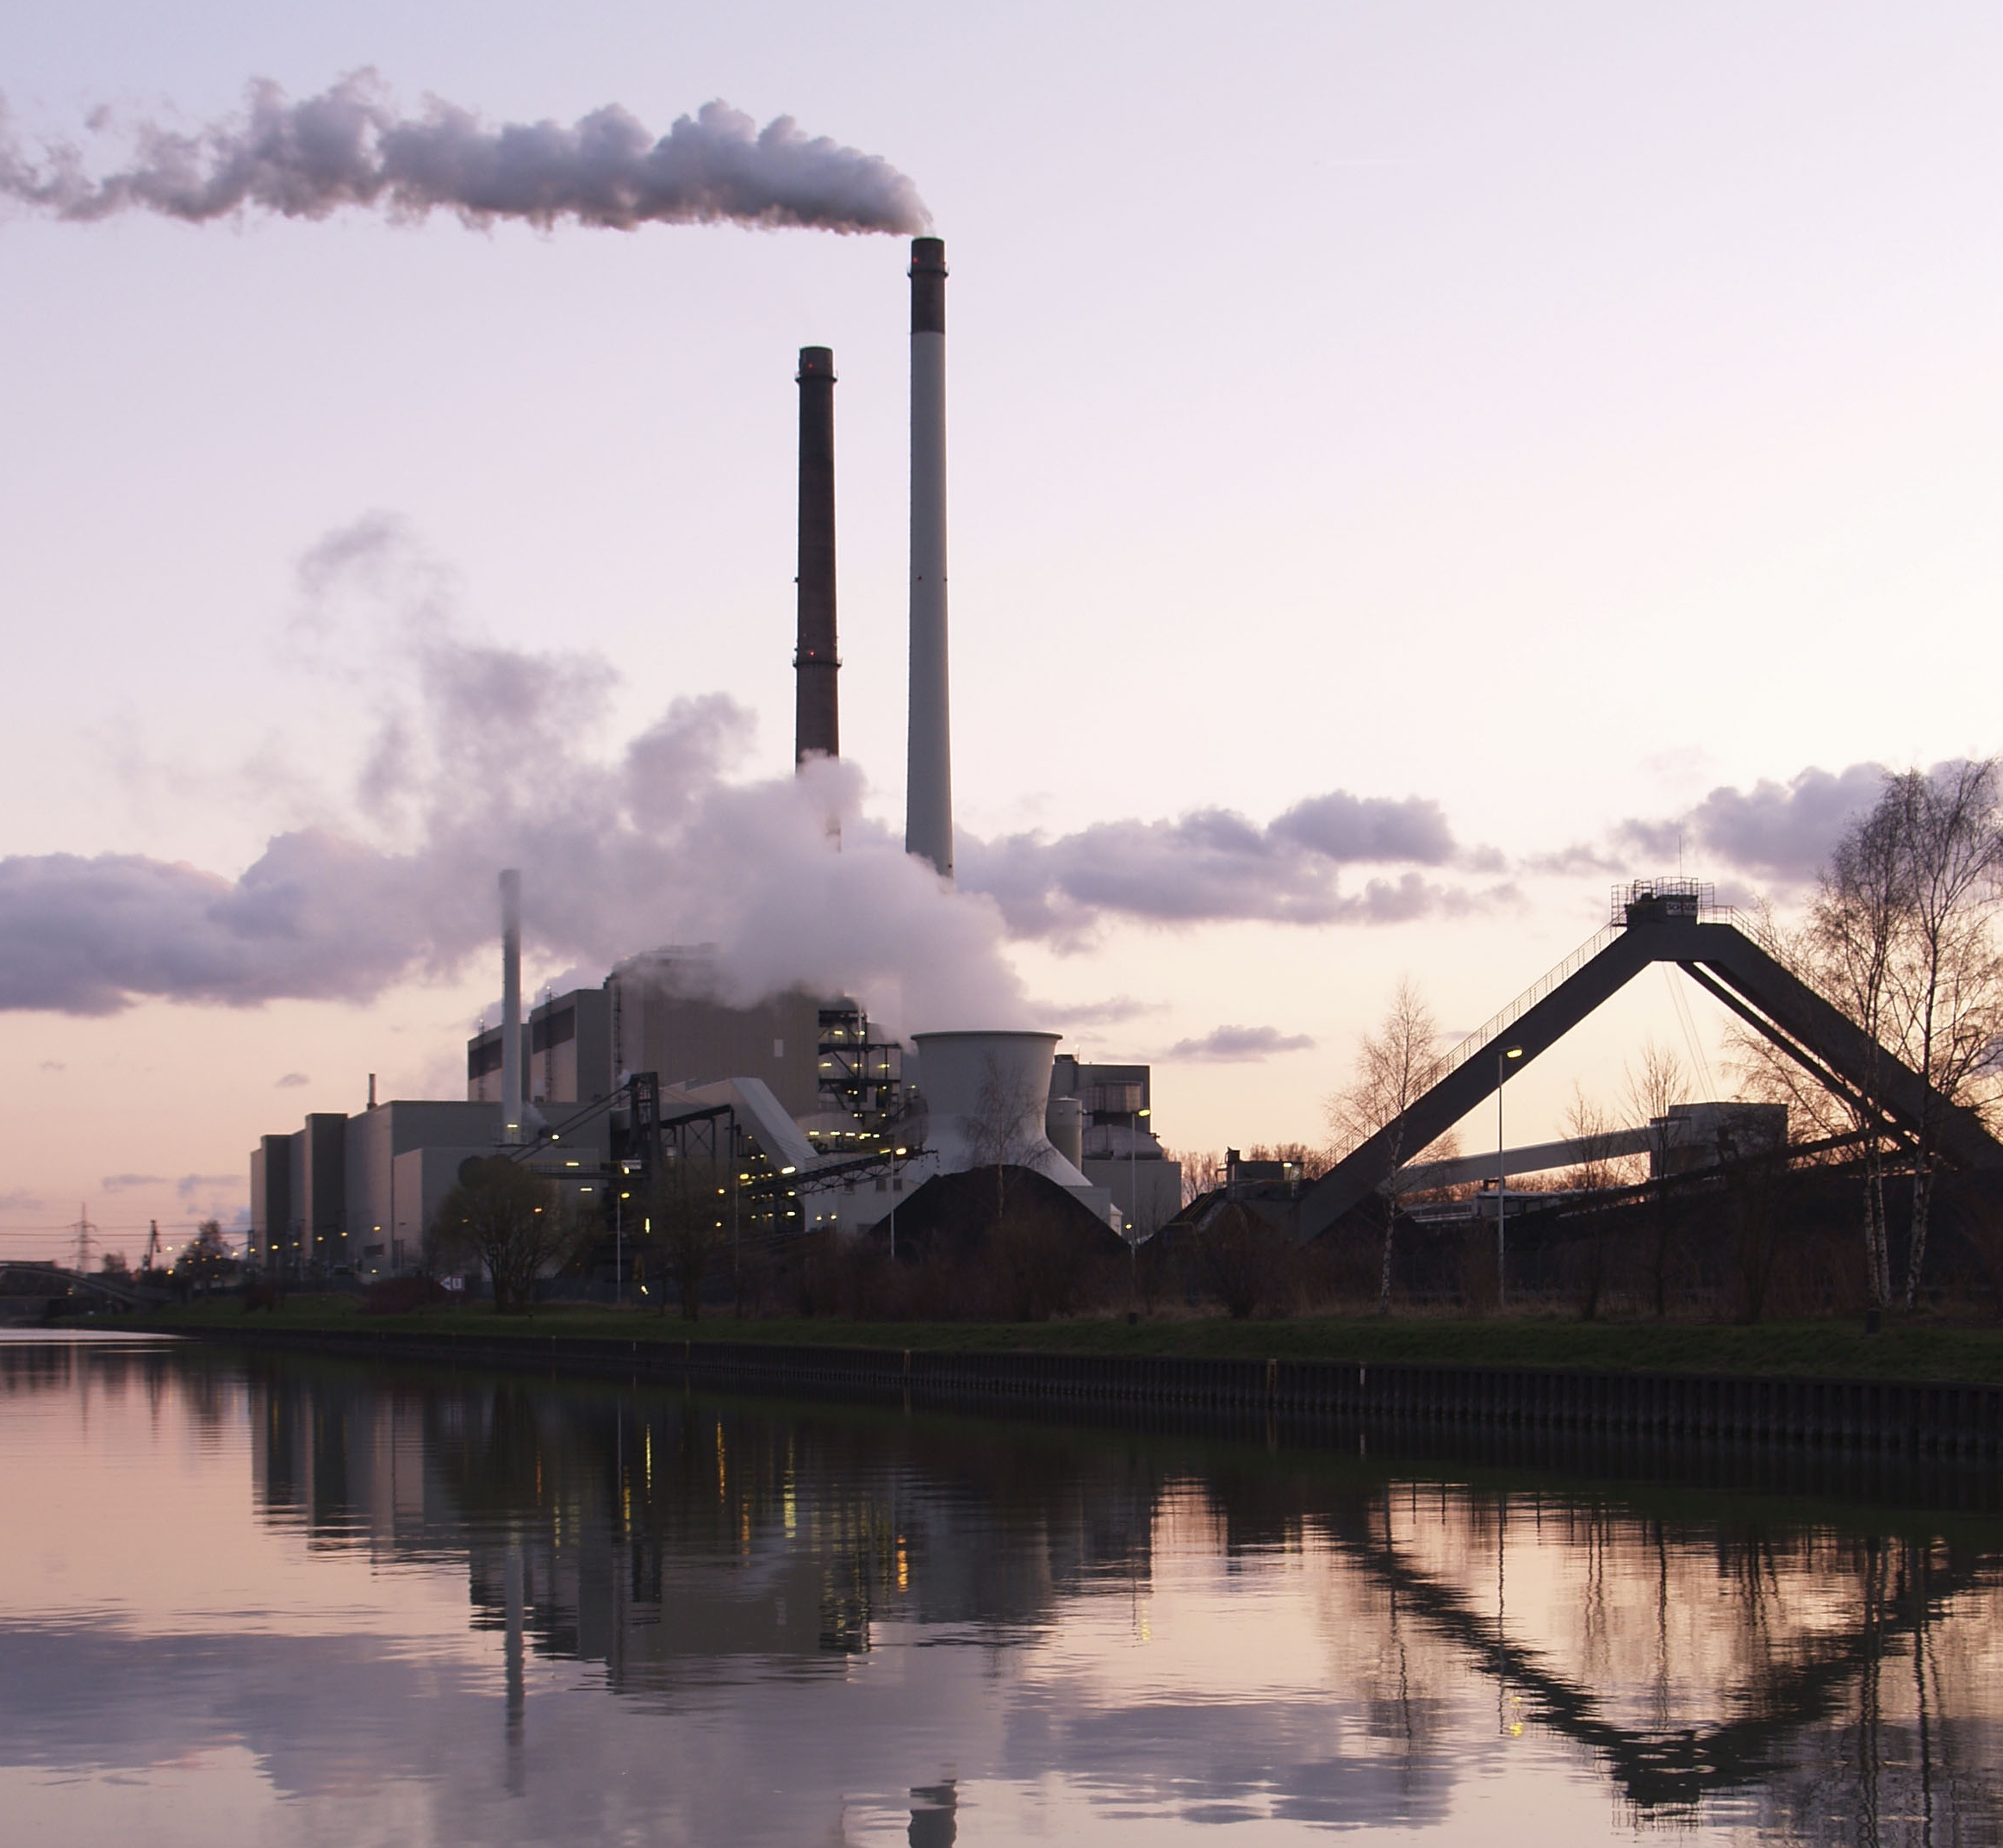
\includegraphics{figures/pollution1.png}

\hypertarget{section}{%
\subsection{}\label{section}}

¡El debate en Biología de la Conservación!

Entonces, ¿cuál es más importante para la conservación? ¿El paradigma de
la población en declive o el paradigma de la pequeña población?

Esta ``controversia'' fue iniciada por un \href{caughley1.pdf}{artículo
muy influyente de Graeme Caughley} en \emph{Journal of Animal Ecology }
en 1994.

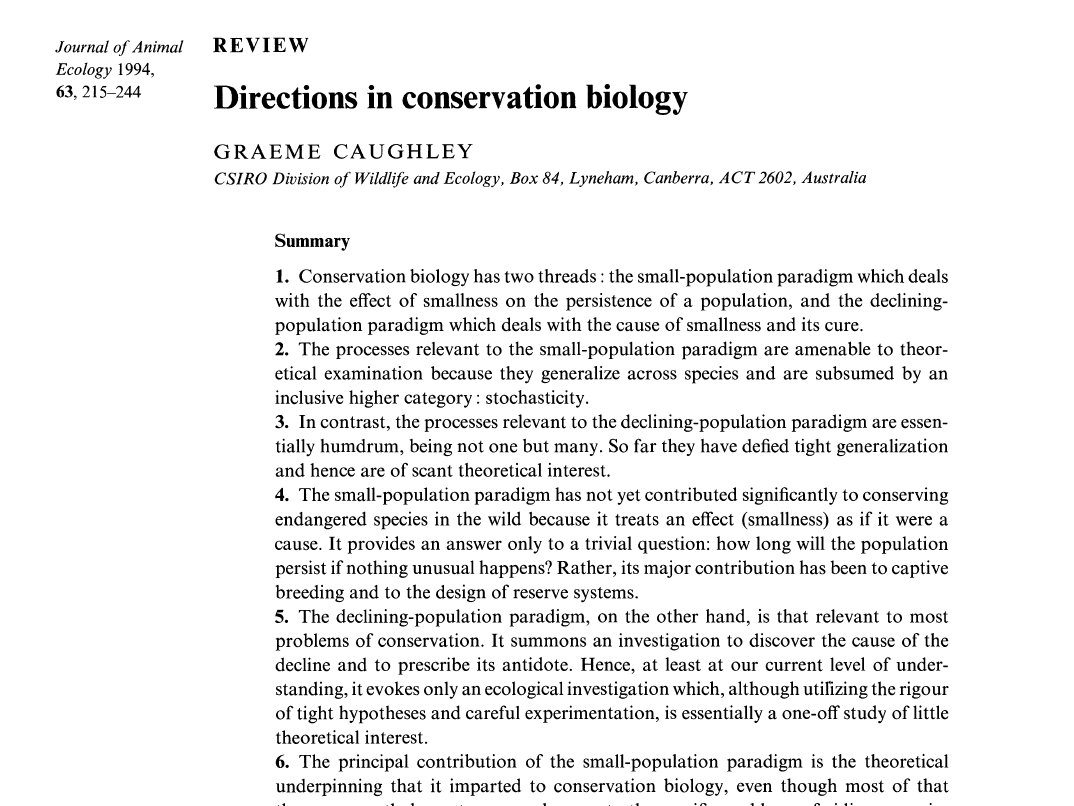
\includegraphics{figures/caughley1.jpg}

En este artículo, Caughley acuñó los términos `paradigma de población
pequeña' y `paradigma de población en declive', y expresó un fuerte
sesgo hacia un paradigma y contra el otro \ldots{}

\emph{La biología de la conservación tiene dos hilos: el paradigma de la
pequeña población, que se ocupa del efecto de la pequeñez en la
persistencia de una población, y el paradigma de la población en
declive, que se ocupa de la causa de la pequeñez y su cura.}

\begin{quote}
Conservation biology has two threads: the small-population paradigm
which deals with the effect of smallness on the persistence of a
population, and the declining- population paradigm which deals with the
cause of smallness and its cure.
\end{quote}

\textbf{Q}: ¿Puedes detectar el sesgo de Caughley en la cita anterior?

\textbf{Q}:¿Qué piensas? ¿Estás de acuerdo con Caughley? ¡Tómese un
momento para revisar el documento y comente en Edmodo!

\hypertarget{ejercicio-en-clase-amenazas-deterministas}{%
\subsubsection{Ejercicio en clase: amenazas
deterministas}\label{ejercicio-en-clase-amenazas-deterministas}}

Probemos con un ejemplo trabajado para ilustrar los puntos anteriores.

Comencemos con una población escalar y dependiente de la densidad
mejorada; debería verse así:

Puede clonar este modelo haciendo clic en
\href{https://insightmaker.com/insight/74417/declining-population-paradigm}{here}

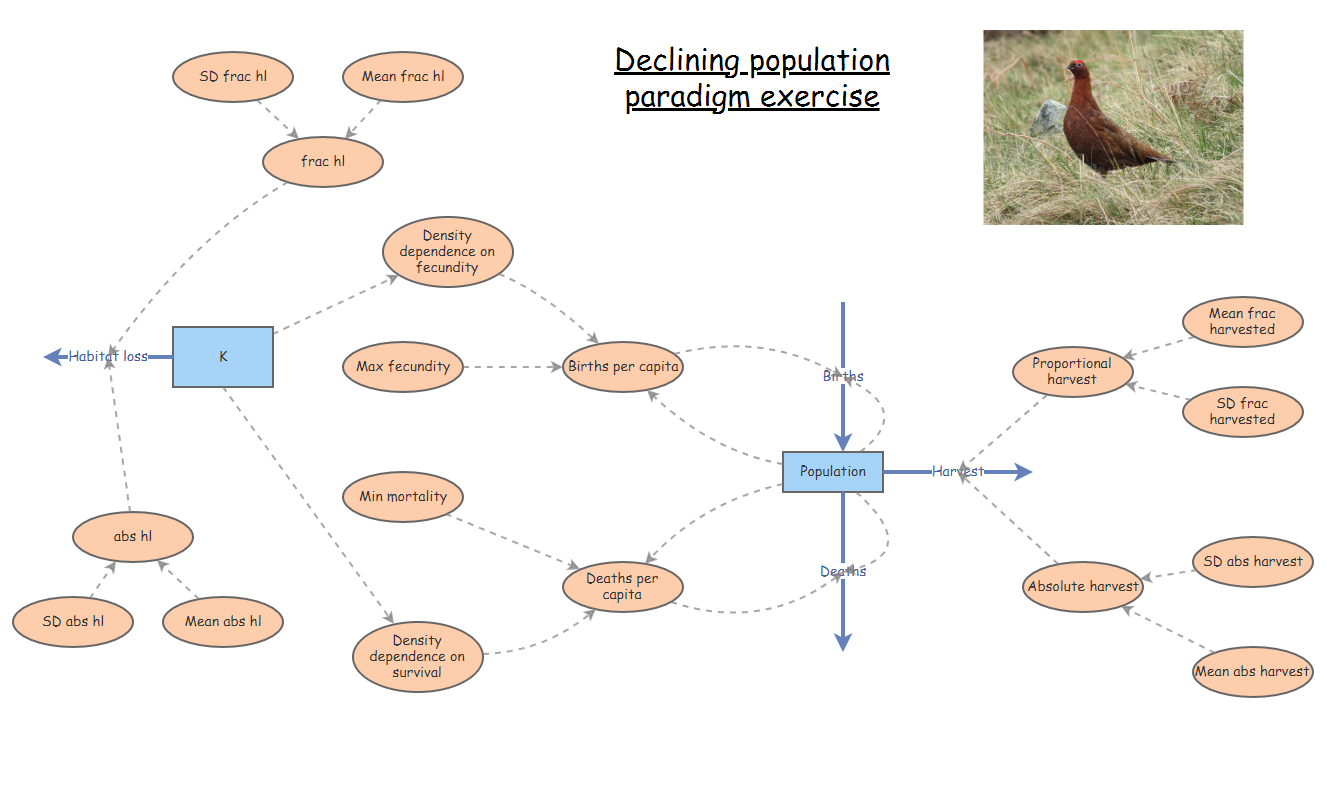
\includegraphics{figures/IM5.PNG}

Debería ver un crecimiento logístico (con estocasticidad demográfica) si
presiona el botón de simulación. Tómese un minuto para ejecutar el
modelo base y asegúrese de comprender cómo funciona.

Para este ejercicio, cambiemos la población inicial a 200 (la mitad de
K).

Además, asegúrese de que el intervalo de tiempo sea de 1 año y que el
modelo deba funcionar durante 50 años.

\textbf{Agreguemos un proceso de cosecha!}

\begin{itemize}
\tightlist
\item
  Suponga que aproximadamente el 10\% de la población se cosecha cada
  año (una cosecha fraccionada). Sin embargo, la verdadera tasa de
  cosecha es estocástica y \emph{normalmente distribuida} -
  ocasionalmente la cosecha llega hasta el 15\% y ocasionalmente hasta
  el 5\%. Asegúrese de especificar los parámetros de `cosecha
  fraccionada' (media y stdev) en el modelo para lograr este rango.
\end{itemize}

\textbf{Q}: ¿Qué valor usó para la desviación estándar de la
distribución normal?

\textbf{Q}: ¿Se considera mejor esta variación en la tasa de cosecha
como un tipo de \emph{estocasticidad demográfica } o un tipo de
\emph{estocasticidad ambiental }?

\textbf{Q}: ¿Por qué la población no desciende hasta la extinción? ¿Qué
ha hecho el proceso de cosecha en este caso?

\textbf{Q}: ¿Qué pasa si cambia la tasa de cosecha, la hace aún más
extrema? Comenzando con una abundancia de 200, ¿cuál es la abundancia
final esperada (después de 50 años) si la tasa de cosecha es del 40\% y
la variación (desviación estándar) en la tasa de cosecha es del 20\%?
{[}Edmodo{]}

\textbf{¡Agreguemos un proceso de pérdida de hábitat!}

Tenga en cuenta que estamos modelando la pérdida de hábitat como una
disminución en la capacidad de carga. Para hacer esto, imponemos
términos de dependencia de densidad más amplios sobre la supervivencia y
la fecundidad: debido a que hay menos hábitat, los efectos del
hacinamiento son más pronunciados.

\begin{itemize}
\item
  Elimine cualquier proceso de cosecha fraccional por ahora (establezca
  los términos de cosecha fraccionada en 0)
\item
  Primero modelemos el caso donde el 10\% de K se pierde cada año
  (pérdida fraccional de hábitat).
\item
  ¡Ejecute la simulación para realizar un seguimiento visual de K junto
  con la dinámica de la población!
\end{itemize}

\textbf{P }: ¿Parece realista la reducción de K a lo largo del tiempo?
¿Puedes imaginar otras formas plausibles para esta curva?

\begin{itemize}
\tightlist
\item
  Intente ejecutar el modelo con un 10\% de pérdida de hábitat (pérdida
  de hábitat fraccional) Y 10\% de recolección (recolección fraccionada
  y pérdida de hábitat fraccional).
\end{itemize}

\textbf{P }: ¿Los resultados son diferentes a los que esperaba?

\begin{itemize}
\item
  Intente cambiar el proceso de cosecha para que sea de 35
  \emph{individuos } por año (tasa de cosecha absoluta). ¿Lo que sucede?
  Regrese la cosecha absoluta a cero.
\item
  Intente cambiar el proceso de pérdida de hábitat para que sea de 5
  \emph{individuos } por año (pérdida absoluta de hábitat). ¿Lo que
  sucede?
\item
  Intente cambiar el proceso de pérdida de hábitat para que sea de 5
  \emph{individuos } por año (pérdida absoluta de hábitat) Y el proceso
  de recolección para que sea de 35 \emph{individuos } por año (tasa de
  recolección absoluta). ¿Lo que sucede? {[}Edmodo{]}
\end{itemize}

\textbf{P }: Pruebe diferentes combinaciones de amenazas deterministas
(¡amenazas en competencia!). ¿Puede identificar algunas combinaciones
que sean \emph{sinérgicas }, es decir, que afecten la disminución de la
población o el riesgo de extinción más que simplemente agregar los
efectos de cada amenaza de forma aislada?

\textbf{P }: ¿Importa más la estocasticidad en las tasas de
aprovechamiento que la estocasticidad en la pérdida de hábitat? ¿O
viceversa?

\href{LECTURE12.html}{--go to next lecture--}

\end{document}
